\chapter{Background}

In this chapter we compare streaming data flow architectures with
traditional, general purpose architectures and we describe the Maxeler
hardware acceleration solution and the MaxCompiler toolchain and API
which represent the target of the MaxC compilation process. We also
look at the LARA language which will be used as part of the design
flow to specify and apply optimization strategies both to the original
source code and to the resulting dataflow design. We also present some
of the related work in the areas of high level synthesis tools,
dataflow languages and aspect-driven compilation for FPGA designs.

\section{Dataflow Computing}

Although general purpose computing devices offer a convenient
programming paradigm, the traditional fetch - decode - execute cycle
is inherently sequential and relies on inefficient access to external
memory. To compensate for this a large area of a modern CPU core is
dedicated to caches, branch prediction units and out-of-order
scheduling and retirement units. This reduces the area of the chip
available for performing useful computation. Furthermore, although
multicore programing is an answer for the processor power wall (which
prevents increases in operating frequency beyond a certain point,
limiting the processing speed of a single core device), there are
classes of algorithms whose performance does not scale linearly with
the number of cores. This is especially true when operating on large
volumes of data with poor spatial locality that do not fit into a
CPU's on-chip cache such as algorithms involving sparse matrix
computations or convolution
\cite{Lindjtorn:Clapp:Pell:Mencer:Flynn:2010}. Although this model
offers good flexibility when dealing with arbitrary access patterns,
it is not efficient for large volumes of highly regular data.

The dataflow computing paradigm operates differently form the general
purpose computing paradigm (as shown in Figure \ref{fig:cpudfe}),
being designed to be efficient at processing large volumes of data. It
works by creating a streaming dataflow graph of computational nodes,
which operates as a large computational pipeline: input data is
streamed in sequentially through each pipeline stage and output data
is streamed out. This results in a highly pipelined design that can be
statically scheduled achieving throughput rates of one value per cycle
by completely avoiding pipeline hazards. This means that a design
running at a few hundred megahertz can outperform a CPU implementation
running at a few gigahertz while being more energy efficient
\cite{Pell:Mencer:2011}.


\begin{figure}[h] \centering
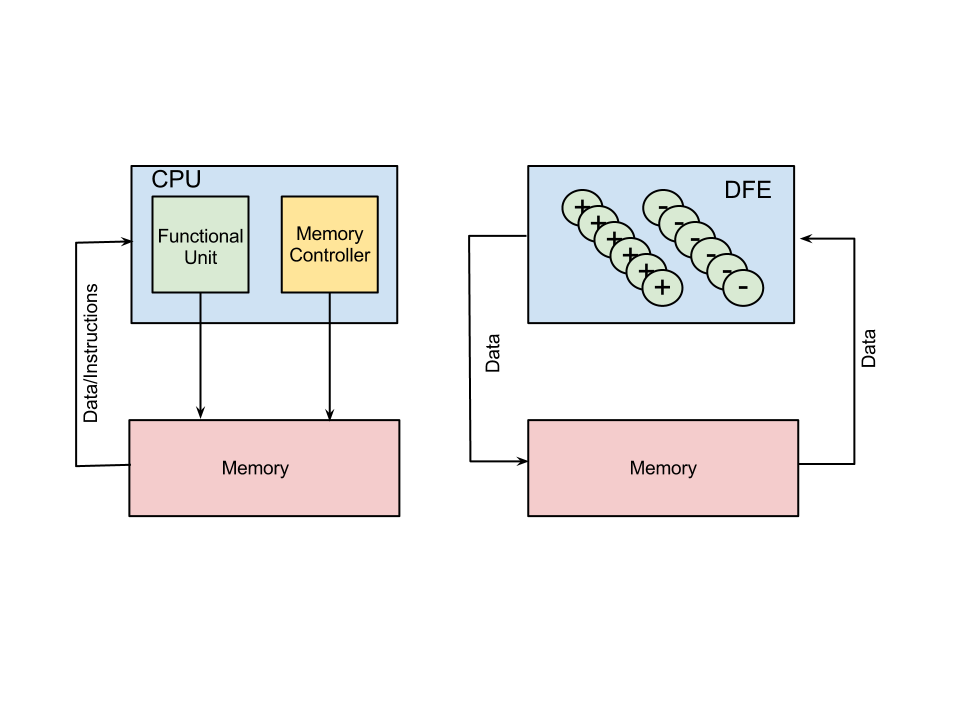
\includegraphics[scale=0.4, trim=0 200 0 150]{figs/cpu-vs-dfe.png}
\caption{Comparison between general purpose CPU architecture and a
streaming Data Flow Engine. In the case of the latter instructions are
not stored in memory but encoded in the dataflow graph. }
\label{fig:cpudfe}
\end{figure}

\section{Maxeler Acceleration Platform}

Maxeler Technologies provides a software and hardware acceleration
solution based on the dataflow computing model. The dataflow design is
created using MaxCompiler \cite{Maxeler} and implemented on a specialized
hardware platform, built around high-end Field Programmable Gate Array
(FPGA) chips.

FPGAs are logic chips that can be reconfigured in seconds to implement
custom applications. Hence they offer a much shorter time to market
than traditional ASIC\footnote{Application Specific Integrated
  Circuit} based solutions, while still being able to implement custom
logic circuits, making them significantly faster than general purpose
hardware. However, the size of the FPGA chip constrains the design
that can be uploaded onto the chip. FPGAs have a limited number of
each of the following resource types:

\begin{itemize}
\item look-up tables (LUTs) - implement the logical functions performed by the circuit;
\item flip-flops (FFs) - small storage elements;
\item digital signal processors (DSP) - small special purpose arithmetic units;
\item block RAM (BRAM) - larger, on-chip storage elements.
\end{itemize}

The specific data flow engine used for this project is a MAX3424A card
based on a Virtex 6 FPGA chip \cite{Virtex6}. The MAX3 provides 24GB of
on-board DRAM and about 4MB of fast on-chip BRAM are available on the
FPGA chip.

The system is connected to the dataflow engine via PCIe as shown in
Figure \ref{fig:max3}.

\begin{figure}[h]
\centering
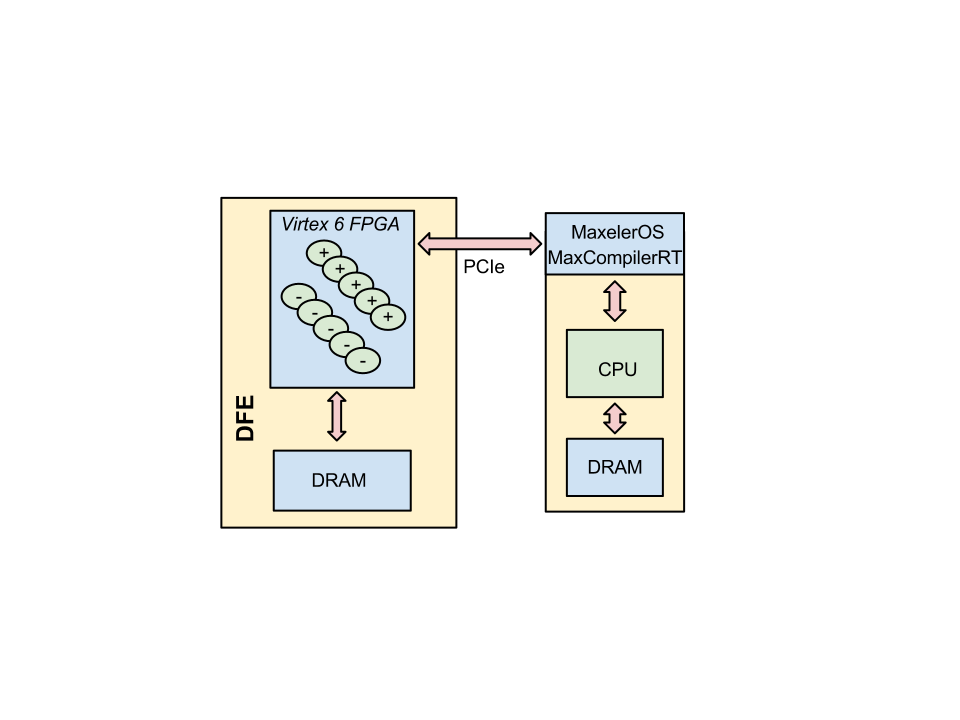
\includegraphics[scale=0.4, trim=0 200 0 200]{figs/max3.png} \caption{
The Maxeler acceleration solution: the DFE is connected to
the host machine via PCIe. The board comprises 48GB of DRAM and a
Virtex 6 FPGA chip. }
\label{fig:max3}
\end{figure}


Since the target of our compilation process is a MaxJ/MaxCompiler
design, we provide a brief summary of the most important features in
the rest of this section.

We demonstrate the use of MaxCompiler in accelerating a simple moving
average computation, starting from an original design in C shown in
Listing \ref{MovingAvg-C}. This performs a three point moving average
computation on an input array x, using 2 point averages at boundaries.

\begin{lstlisting}[
language=C++,
caption={Original three point moving average computation in C.},
label={MovingAvg-C}]
for (int i = 0; i < n; i++ ) {
   sum = x[i], divisor = 1;
   if ( i > 0 )
     sum += x[i - 1], divisor++;
   if (i < n - 1)
     sum += x[i + 1], divisor++;
   y[i] = sum / divisor;
}
\end{lstlisting}

\subsection{MaxJ}

MaxJ is a high-level language for specifying dataflow
architectures. It is largely based on Java and adopts a
meta-programming approach for specifying dataflow graphs.  Listing
\ref{lst:moving-avg-kernel} shows the dataflow kernel for computing a
three point moving average over an input stream, which highlights some
of the important features of the MaxJ language:

\begin{itemize}

\item kernel inputs and outputs provide an I/O interface that allow
  the kernel to communicate with the rest of the design (Lines
  \ref{lst:mak-in} and \ref{lst:mak-out});

\item stream offset expressions allow accessing past and future
  elements of a stream (Lines \ref{lst:mak-off} and
  \ref{lst:mak-off2}). The offset window is stored into on chip BRAM
  so is limited to a few tens of thousands elements;

\item frequently used components such as counters are provided by the
  API. They are useful in keeping track of iteration count when
  mapping loops to streaming designs (Line \ref{lst:mak-counter});

\item operator overloading is used to perform arithmetic on input streams;

\item multiplexers (in this instance represented by the overloaded
  conditional operator) are used to select between streams (Lines 11
  and 12).

\end{itemize}

\begin{lstlisting}[
language=Java, style=MaxJ, label={lst:moving-avg-kernel},
caption={Kernel design for the three point moving average computation showing features such as stream offsets, arithmetic and control which will have to be supported by our MaxC language}
]
public class MovingAverageKernel extends Kernel{
  public MovingAverageKernel(...) {
    super(...);
    HWVar x = io.input("x", hwFloat(8, 24)); (*@\label{lst:mak-in}@*)
    HWVar cnt = control.count.simpleCounter(32, N); (*@\label{lst:mak-counter}@*)

    HWVar prev = cnt > 0       ? stream.offset(x, -1) : 0; (*@\label{lst:mak-off}@*)
    HWVar next = cnt < (N - 1) ? stream.offset(x, +1) : 0; (*@\label{lst:mak-off2}@*)
    HWVar divisor = cnt > 0 & cnt < (N - 1) ? 3.0 : 2.0;

    HWVar y = (prev + x + next) / divisor;
    io.output("y" , y, hwFloat(8, 24) ); (*@\label{lst:mak-out}@*)
  }
}
\end{lstlisting}

\subsection{MaxCompiler}

\label{sec:back--maxcompiler}

MaxCompiler~\cite{5719584} is a high level compiler targeting the
acceleration platform developed by Maxeler Technologies. It provides a
Java based API for specifying hardware designs that are compiled and
uploaded onto the DFE and a C runtime interface (MaxCompilerRT and
MaxelerOS shown in Figure \ref{fig:max3}) for the part of the
application running on the CPU of the host system.

In addition to the dataflow kernels, a MaxCompiler design also
contains a manager design which is sude manage kernel I/O, connecting
multiple kernels together (in multi kernel designs) and kernels to
DRAM and the CPU interface (via PCIe).

A number of dataflow kernels are connected via a manager to create a
dataflow design which is then compiled to the a Xilinx bitstream that
can be uploaded to the FPGA. Additionally a number of run-time
functions are generated that can be called by the MaxCompiler run-time
to load the design and initiate the streaming of data to and from the
dataflow design.

An example manager design is shown Listing
\ref{lst:moving-avg-manager} and is used to instantiate a single
moving average kernel and connect its inputs and outputs to the host
interface.

\begin{lstlisting}[
language=Java,
label={lst:moving-avg-manager},
 caption={Manager design for the
three point moving average computation}
]
public class MAManager extends CustomManager {
  public MovingAverageManager(...) {
    super(...);
    KernelBlock k = addKernel(new MovingAverageKernel(...));
    k.getInput("x") <== addStreamFromHost("x");
    addStreamToHost("y") <== k.getOutput("y");
  }
}
\end{lstlisting}

\subsection{Run-time}
Finally we must write a host application which is required to queue
the input streams and run the accelerator. This is achieved by calls
to the MaxCompilerRT (runtime) API that interfaces with MaxelerOS.

\begin{lstlisting}[
label={MovingAverage-Host},
caption={Host example for queueing
the input and output streams and running the three point moving
average design.}
]
max_run(
  device,
  max_input("x", x, x_size),
  max_output("y", y, y_size),
  max_runfor("MAKernel", n),
  max_end());
\end{lstlisting}

\subsection{Analysis}
Although the MaxCompiler toolchain greatly simplifies the process of
accelerating applications and particularly the designing of dataflow
kernels, the acceleration process is still very involved and requires
a large amount of experience with FPGA technology and domain specific
knowledge. Most importantly the whole process is manually driven
including the exploration of optimizations. This step is a critical
and time consuming part of the design process which is vital in
achieving maximum performance (in terms of operating frequency, number
of parallel pipelines etc.) subject to physical limitations such as
chip size or timing constraints.

By specifying the design in \FAST{} and optimization strategies in LARA
we aim to create the basis of a design space exploration flow that can
automate this process.

\section{Aspect Oriented Programming}

\subsection{LARA}

Lara is an aspect oriented programming language for specifying
compiler strategies for FPGA-based systems
\cite{Cardoso:Teixeira:Alves:Nobre:Diniz:Cutinho:Luk:2012}. The key
feature of the LARA aspect-oriented approach is that it separates the
application code from the strategies required to compile and optimize
it for a particular platform. It enables the capturing of strategies
for:

\begin{itemize}
\item instrumentation, monitoring and hardware-software partitioning --
  these will be used in the initial stages of our proposed design flow
  to identify optimization candidates for mapping onto the accelerator

\item code specialization and code optimization -- these will be
  used both for the original source code application which is the
  target of the compilation and for the dataflow design
\end{itemize}

Furthermore LARA descriptions can be parametrized which facilitates
integration with our proposed DSE step described in Chapter
\ref{sec:design_flow}.

Listing \ref{lara} shows an example description used for fully
unrolling all innermost loops with an iteration count smaller than or
equal to 16. The `select` statement on line 2 captures the join points
on which the aspect acts, the `apply` statement specifies actions to
be applied to the results of a query while `condition` is used to
filter relevant queries.

\begin{lstlisting}[
style=lara,
label={lara},
caption={Example LARA description
for fully unrolling innermost loops with an iteration count smaller
than or equal to 16.}
]
aspectdef loopunroll
  select function.loop{type="for"} end
  apply optimize("loopunroll", "fully"); end
  condition $loop.is_innermost && $loop.num_iter<=16; end
end
\end{lstlisting}

\cite{Cardoso:Carvalho:Teixeira:Diniz:Goncalves:Petrov:2012} also
introduces a design flow based on LARA for mapping applications into
heterogeneous multicore platforms. This involves specifying
optimizations and mapping strategies in the LARA programming language,
separate from the application source code.

The strategies are compiled and applied to the original source code in
a sequential order to obtain the final design which is synthesized
using Catapult-C \cite{CatapultC}. Examples of strategies which are
expressed using LARA include loop unrolling, coalescing, loop fission
and mapping compute intensive functions to hardware (hardware/software
partitioning).

Advantages of the aspect based approach compared with the popular
pragma based approach used in frameworks like
OpenMP \cite{Ferrer:Judit:Bellens:Duran:Gonzalez:Marorell:Badia:Ayquade:Labarta:2011}
include the possibility of defining dynamic join points through which
strategies can be applied to the intermediate results of the weaving
(source translation) process. Additionally optimization strategies are
grouped into cohesive aspects, rather than being spread through the
code which makes them easier to understand, maintain and modify, for
example to target a different platform.


\section{Related Work}

\subsection{High Level Synthesis}

Substantial work has been carried out in synthesizing high level
languages to hardware designs and many tools exist for this purpose
\cite{CtoVerilog, Vivado, ImpulseC}. However these approaches
do not target a streaming dataflow architecture but either soft
processor designs - processor cores implemented on the FPGA chip with
configurable custom computing units (e.g. floating point units). These
usually offer limited speedups when compared to high-end hardcore
CPUs but can turn out to be more energy efficient.

\cite{Czerniawski} proposes a method for synthesising hardware
pipelines from OpenCL programs which exploits some important concepts
related to parallelism exposed by the OpenCL specification
\cite{OpenCL} such as threads and domain decomposition into threads
sharing local memory. Although we are dealing with simple C kernels
for this project, some of the proposed compilation strategies can be
applied for loops.

\subsection{Dataflow Languages}
A number of dataflow languages have been developed targeting FPGAs but
also multi-core platforms. Table \ref{table:feature-comparison}
summarises some of the important features of these languages compared
to \FAST{}.

Lucid~\cite{ashcroft1977lucid},
SISAL~\cite{gurd1987implicit,mcgraw1983sisal}, and
Lustre~\cite{halbwachs1991synchronous}, are examples of functional
dataflow languages. The latter is based on a synchronous programming
model, facilitating safety verification for critical
software~\cite{halbwachs1992programming} rather than performance. The
functional programming style complicates the translation of existing
imperative applications and none have existing implementations for
FPGAs, so a performance comparison is not possible.

Streams-C~\cite{Gokhale:Stone:Arnold:Kalinowski:2000} and
ImpulseC~\cite{ImpulseC} adopt imperative ANSI C syntax and an
execution model based on Communicating Sequential Processes and
introduce non-standard syntax and constructs for specifying designs
such as special comment blocks which are used to annotate the C
application code. The specialised syntax makes the languages harder to
integrate with existing source-to-source translation or aspect weaving
frameworks.

Hybrid approaches such as MaxCompiler~\cite{5719584} separate the CPU
run-time component from the accelerated one, providing a C run-time
environment and a Java API for building dataflow designs via
meta-programming. The separation complicates the development process,
hindering sharing of design parameters and, consequently, the design
space exploration process. The use of meta-programming simplifies
design parametrisation, but can make resulting programs harder to
understand. In contrast, the proposed approach allows the computation
description, which includes CPU and dataflow components, to be specified
using a single language and to be decoupled from design
parametrisation and other optimisation strategies which are captured
as LARA aspects. This separation of concerns results in more intuitive
and maintainable descriptions.


\begin{sidewaystable}[!ht]
  \renewcommand{\arraystretch}{2.1}
  \centering
  \label{table:feature-comparison}
  \begin{tabularx}{\textwidth}{ m{2.5cm} | p{2.5cm} | p{3cm} | p{1.9cm}| p{2.8cm} | p{3.2cm} | p{2.5cm}}
    \hline
    \bf{Language}                 & \bf{Syntax}              & \bf{Paradigm}                            & \bf{Support}              & \bf{Implementation}             & \bf{Design Parametrisation}                     & \bf{Optimisation Strategies}            \\
    \hline \hline
    \bf{Lucid}                    & Lucid                    & Functional                               & \multirow{3}{*}{Software} & \multirow{3}{*}{Multiprocessor} & \multirow{3}{3cm}{Manual Source Transformation} & \multirow{5}{3cm}{Manual Code Revision} \\
    \cline{1-3}
    \bf{SISAL}                    & SISAL                    & Functional                               &                           &                                 &                                                 &                                         \\
    \cline{1-3}
    \bf{Lustre}                   & Lustre                   & Synchronous                              &                           &                                 &                                                 &                                         \\
    \cline{1-6}
    \bf{MaxCompiler}              & C99(SW) Java(HW)         & Imperative(SW) Dataflow(HW)              & \multirow{6}{*}{Combined} & \multirow{6}{*}{CPU + FPGA}     & Meta-programming                                &                                         \\
    \cline{1-3}\cline{6}
    \bf{Streams-C} \bf{ImpulseC}\ & C99                      & Imperative(SW) CSP(HW)                   &                           &                                 & Compiler \newline Directives                    &                                         \\
     \cline{1-3}\cline{6-7}
    \bf{\FAST{}}/\bf{LARA}        & C99(SW/HW) LARA(Aspects) & Imperative(SW) Dataflow(HW) AOP(Aspects) &                           &                                 & \multicolumn{2}{p{5.5cm}}{Compiler Directives + \newline Automated Aspect-Directed Source Transformation} \\
  \end{tabularx}
  \caption{Feature comparison of the \FAST{}/LARA approach and existing dataflow implementations.}
\end{sidewaystable}


\subsection{Aspect-driven Compilation of FPGA Designs}

One attempt at capturing optimisation strategies for FPGA designs
 using aspect descriptions is LARA
 \cite{Cardoso:Carvalho:Cutinho:Luk:Nobre:Diniz:Petrov:2012,
   Cardoso:Carvalho:Teixeira:Diniz:Goncalves:Petrov:2012}, an Aspect
 Oriented language for embedded systems. Aspect descriptions are
 written in the LARA language and automatically applied to the
 original application source to generate optimised versions through
 various transformations that enable and optimise hardware/software
 partitioning \cite{Lam:Coutinho:Luk:2008}. Aspect descriptions can be
 used to specify compilation strategies that result in overall
 speedups of 2 to 6.8 times over software versions
 \cite{Cardoso:Teixeira:Alves:Nobre:Diniz:Cutinho:Luk:2012}, generally
 with high aspect bloat \footnote{ $\text{aspect bloat} =
   \frac{\text{size of transformed code}}{\text{size of original
       code}}$, so a higher aspect bloat is better}
 \cite{Cardoso:Carvalho:Cutinho:Luk:Nobre:Diniz:Petrov:2012}.

The use of LARA aspects in guiding the compilation process of C
applications is described in
\cite{Cardoso:Teixeira:Alves:Nobre:Diniz:Cutinho:Luk:2012} and
\cite{cardoso2011new} but the backend compilation targets a von
Neumann architecture (with a GPP and custom accelerator) unlike the
dataflow architecture proposed in this paper. The approach described
in \cite{Cardoso:Teixeira:Alves:Nobre:Diniz:Cutinho:Luk:2012} and
\cite{cardoso2011new} relies more on high-level source transformation
whereas our approach is based on a systematic design space exploration
process, which enables the analysis of more low-level
optimisations. Finally,
\cite{Cardoso:Teixeira:Alves:Nobre:Diniz:Cutinho:Luk:2012} and
\cite{cardoso2011new} do not consider development aspects which can be
used to improve developer productivity.


The use of aspect-oriented programming for specifying strategies for
run-time adaptation of FPGA designs discussed in \cite{6322875}
differs from the static process considered in this paper in which the
application is partitioned and scheduled at compile time, to achieve
optimised performance as described in
\cite{Xinyu:Qiwei:Luk:Qiang:Pell:2012}. An advantage of our approach
is that an optimised allocation is generated prior to application
execution. However, we lack the flexibility of adapting the design to
varying input conditions.

\section{Summary}

We have provided a brief introduction into the area of dataflow
computing and explained why dataflow acceleration can improve
performance and energy efficiency over traditional software only
solutions. We have introduced the Maxeler platform which will be used
as the backend of the compilation process presented in Chapter
\ref{sec:design-flow} and presented some of the more important
features of the MaxCompiler approach as well as the limitations
associated with it and why we believe that the proposed flow can
improve developer productivity and possibly reveal new opportunities
for design transformation and optimisations. Finally, we introduced
some of the existing dataflow languages and existing work in
aspect-driven compilation for FPGA designs.
